\chapter{Diagrammes}
\label{s:Diagrammes}


\section{Diagramme des fonctionnalit�s}
\label{s:Diagramme_fonctionnalites}

%\begin{figure}[htp]
%   \centering
%   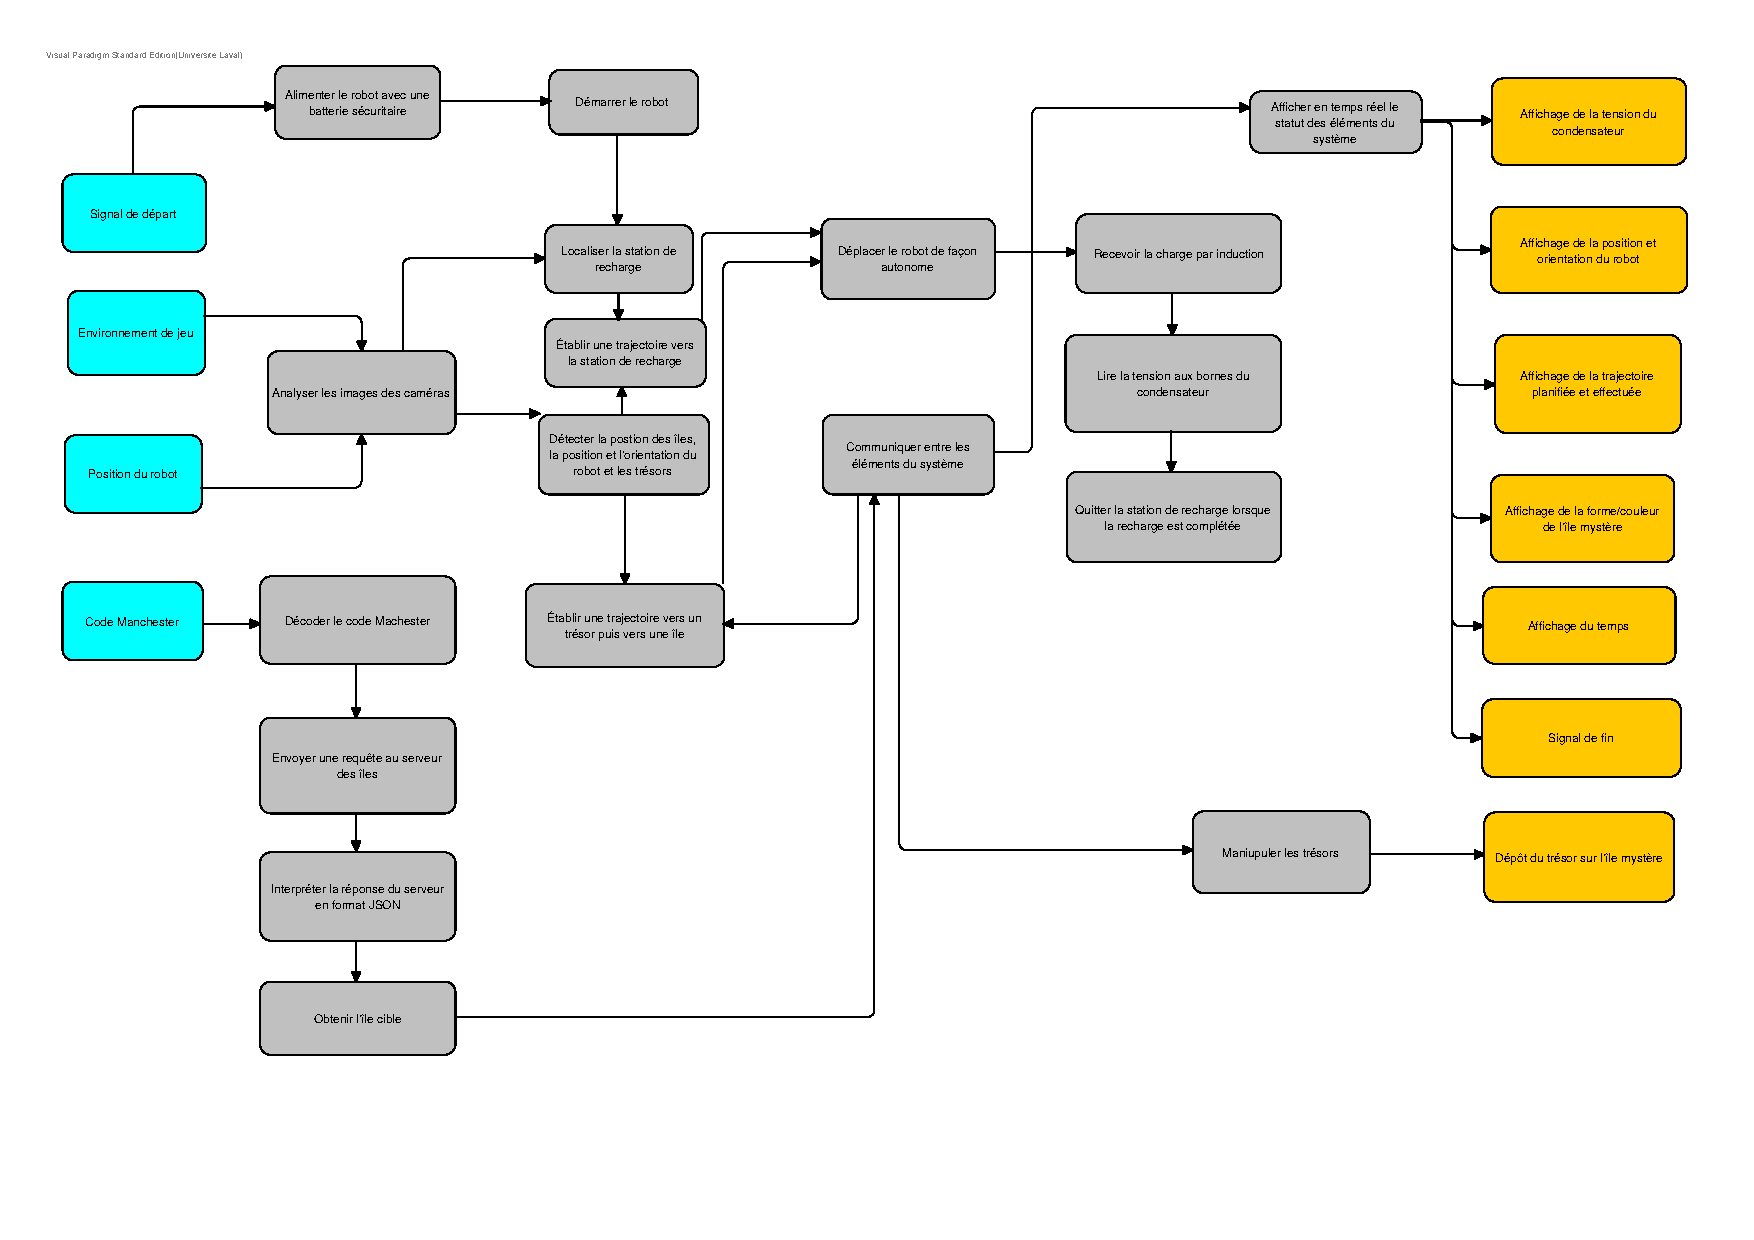
\includegraphics[width=1\textwidth]{pdf/DiagrammeFonctionnalites.pdf}
%   \caption{Diagramme des fonctionnalit�s}
%   \label{f:diagramme_fonctionnalites}
%\end{figure}


%\section{Diagramme physique}
%\label{s:diagramme_physique}

%\begin{figure}[htp]
%   \centering
%   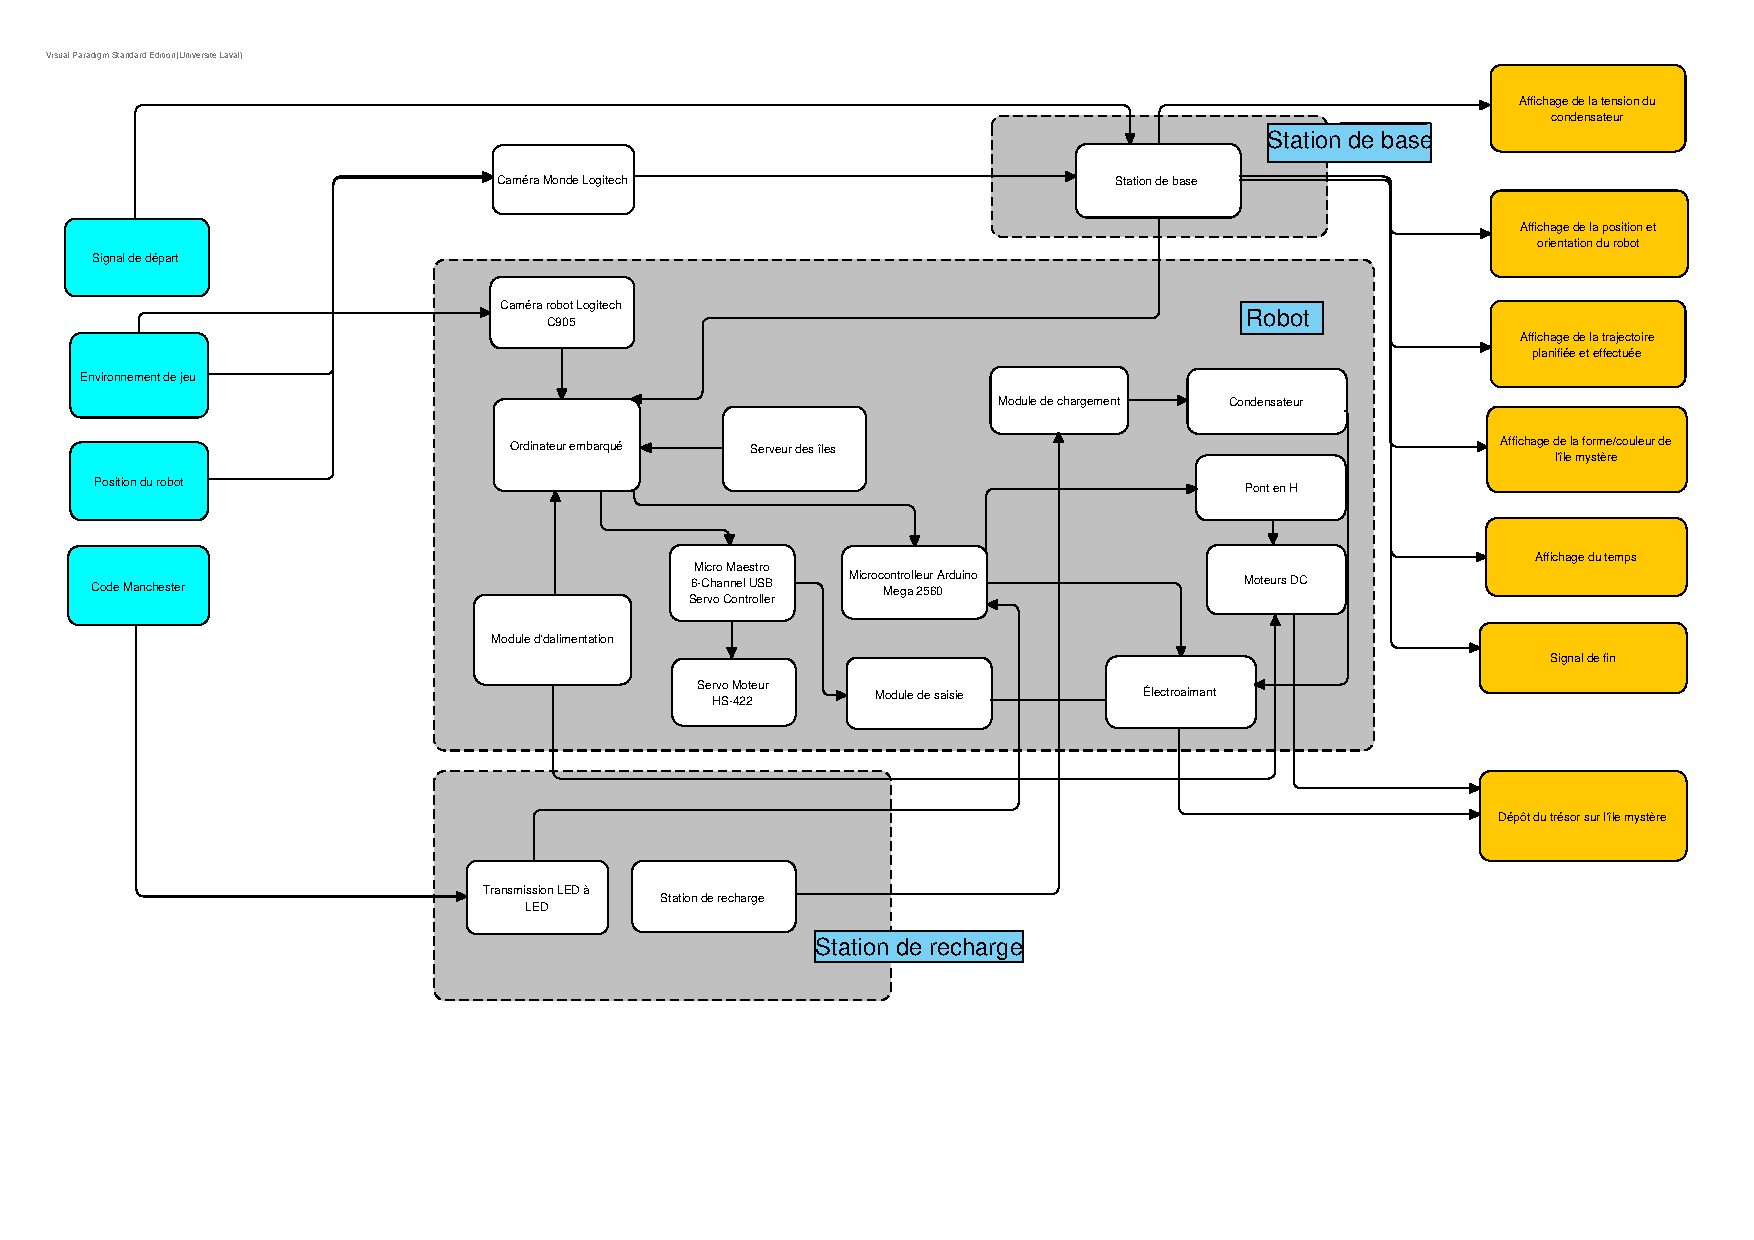
\includegraphics[width=1\textwidth]{pdf/DiagrammePhysique.pdf}
%   \caption{Diagramme physique}
%   \label{f:diagramme_physique}
%\end{figure}

%\section{Diagramme de s�quences}
%\label{s:diagramme_sequence}

%Les figures \ref{f:diagramme_sequence1} � \ref{f:diagramme_sequence4} correspondent aux diagrammes de s�quences.

%\begin{figure}[htp]
%   \centering
%   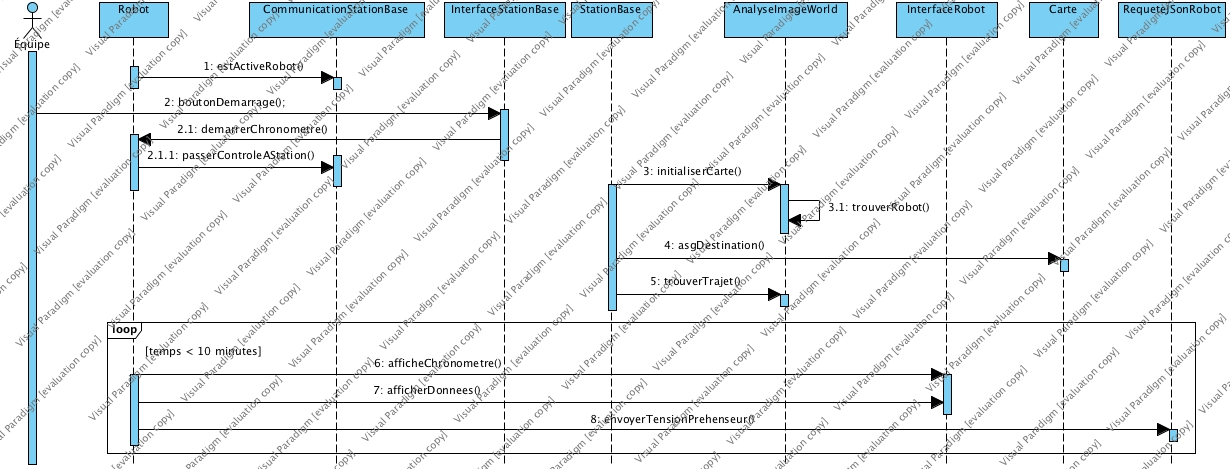
\includegraphics[width=1\textwidth]{fig/demarageRobot.jpg}
%   \caption{Diagramme de s�quences: d�marage du robot}
%   \label{f:diagramme_sequence1}
%\end{figure}

%\begin{figure}[htp]
%   \centering
%   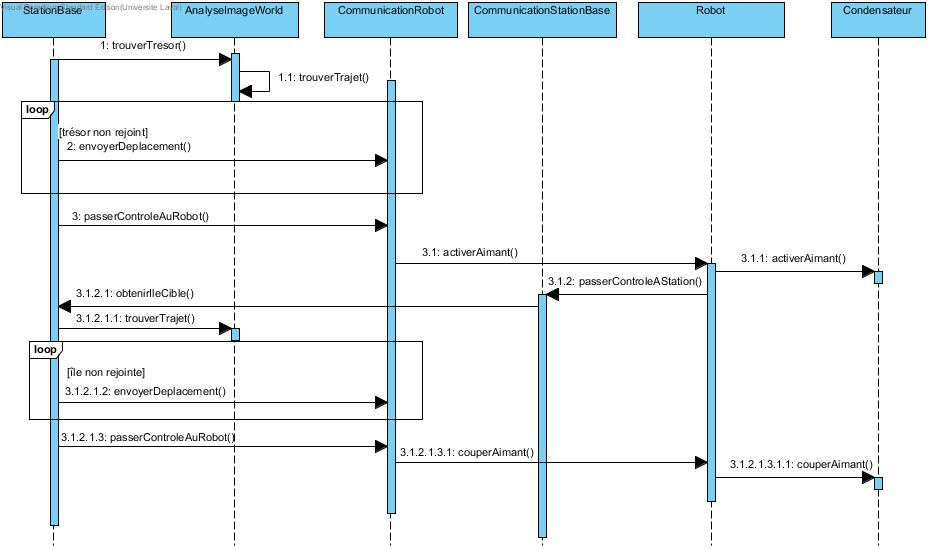
\includegraphics[width=1\textwidth]{fig/deplaceTresor.jpg}
%   \caption{Diagramme de s�quences: Deplacement du tr�sor}
%   \label{f:diagramme_sequence2}
%\end{figure}

%\begin{figure}[htp]
%   \centering
%   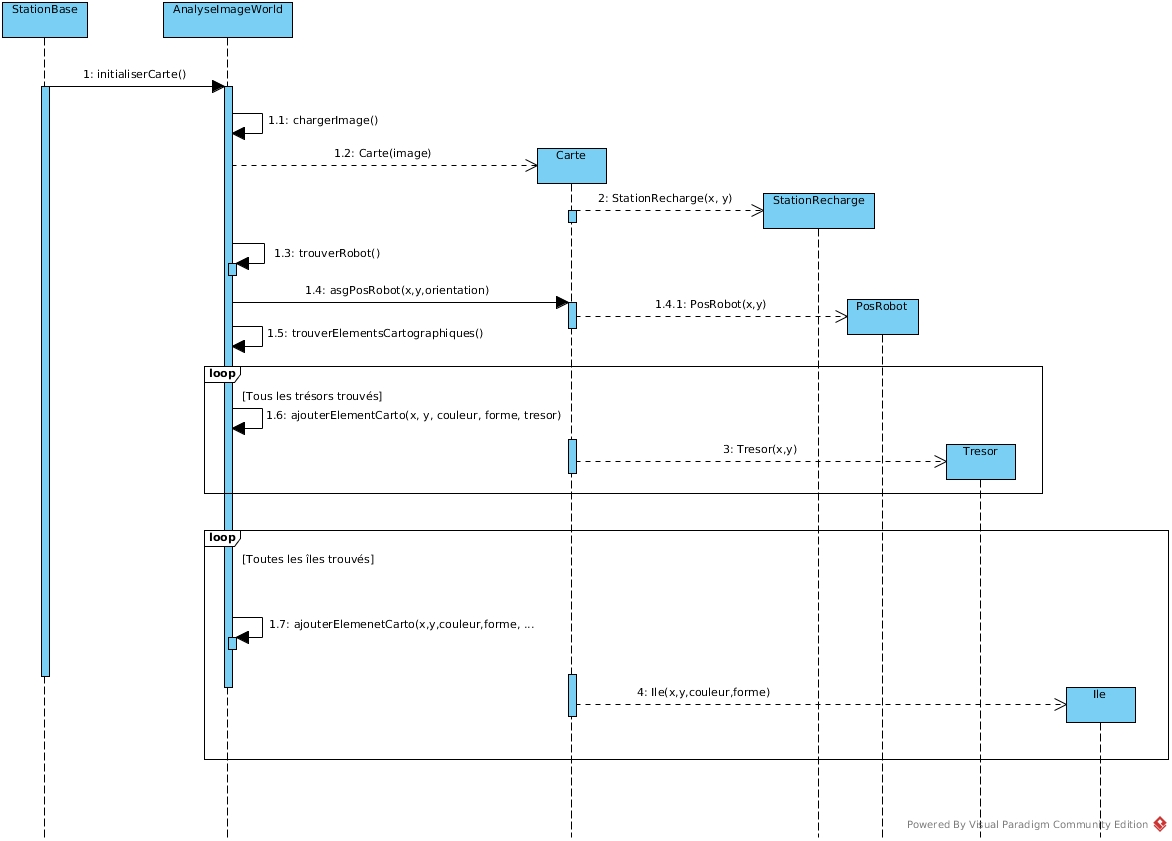
\includegraphics[width=1\textwidth]{fig/initCarte.jpg}
%   \caption{Diagramme de s�quences: initialisation de la carte}
%   \label{f:diagramme_sequence3}
%\end{figure}

%\begin{figure}[htp]
%   \centering
%   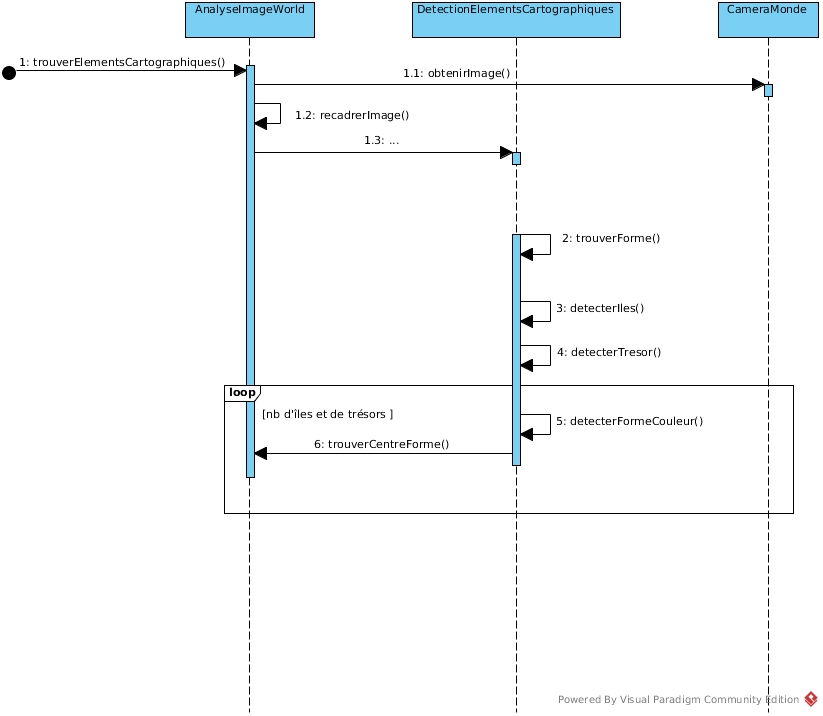
\includegraphics[width=1\textwidth]{fig/trouverIleOuTresor.jpg}
%   \caption{Diagramme de s�quences: trouver les �les et tr�sors}
%   \label{f:diagramme_sequence4}
%\end{figure}
